% =================================================================
% 2026 AstroAI Workshop poster  --  40 x 30 in, landscape
% Jiaming Pan, Nicholas Kern, Dragan Huterer (U. Michigan)
% Compile:  pdflatex astroai_poster.tex   (run from this folder)
% Drop exported notebook PNGs into  figs/  -- slots fill themselves.
% =================================================================
\documentclass{article}
\usepackage[paperwidth=101.6cm,paperheight=76.2cm,margin=1.2cm]{geometry}
\usepackage[T1]{fontenc}
\usepackage{helvet}\renewcommand{\familydefault}{\sfdefault}
\usepackage{amsmath,amssymb,bm}
\usepackage{graphicx}
\usepackage{enumitem}
\usepackage{tikz}
\usetikzlibrary{calc}
\usepackage[most]{tcolorbox}
\usepackage{qrcode}
\pagestyle{empty}
\setlength{\parindent}{0pt}

% ---- Palette (matches the roadmap figure) -----------------------
\definecolor{ink}{HTML}{1B2A4A}
\definecolor{subgray}{HTML}{5A6678}
\definecolor{paramBlue}{HTML}{2E5EAA}
\definecolor{diffPurple}{HTML}{6B4FA0}
\definecolor{fieldTeal}{HTML}{0E7C72}
\definecolor{vggOrange}{HTML}{C25E12}
\definecolor{loopRed}{HTML}{B0303C}
\definecolor{paleBg}{HTML}{F4F6FA}

% ---- Type sizes --------------------------------------------------
\newcommand{\TitleFont}{\fontsize{74}{82}\selectfont\bfseries}
\newcommand{\AuthorFont}{\fontsize{36}{44}\selectfont}
\newcommand{\BoxTitleFont}{\fontsize{34}{38}\selectfont\bfseries}
\newcommand{\BodyFont}{\fontsize{24.5}{31}\selectfont}
\newcommand{\SmallFont}{\fontsize{19}{24.5}\selectfont}

% ---- Section box style -------------------------------------------
\tcbset{
  secbox/.style 2 args={
    enhanced, breakable=false,
    colback=white, colframe=#1,
    boxrule=1.8pt, arc=6mm,
    left=7mm, right=7mm, top=3.5mm, bottom=4mm,
    title={\BoxTitleFont #2},
    coltitle=white, colbacktitle=#1,
    toptitle=3mm, bottomtitle=3mm, lefttitle=8mm,
    drop fuzzy shadow=black!35,
    before skip=0mm, after skip=5mm
  }
}

% ---- Figure slot: shows the PNG if present, else instructions ----
% \figslot{<width>}{<height if placeholder>}{<file>}{<where to export it>}
\newcommand{\figslot}[4]{%
  \IfFileExists{figs/#3}{%
    \centering\includegraphics[width=#1,height=#2,keepaspectratio]{figs/#3}%
  }{%
    \begin{tikzpicture}
      \draw[dashed, line width=2pt, subgray, rounded corners=5mm, fill=paleBg]
        (0,0) rectangle (#1,#2);
      \node[align=center, text=subgray, text width={\dimexpr#1-4cm\relax}] at (0.5*#1,0.5*#2)
        {\SmallFont\bfseries drop in:\ {\ttfamily\detokenize{figs/#3}}\\[3mm]\SmallFont #4};
    \end{tikzpicture}%
  }%
}

\newcommand{\hl}[2]{{\color{#1}\bfseries #2}}

\begin{document}\BodyFont\color{ink}

% ================== HEADER BAND ===================================
\begin{tikzpicture}
  \node[anchor=north west, fill=ink, rounded corners=8mm,
        minimum width=99.1cm, minimum height=10.6cm] (hdr) at (0,0) {};
  \node[anchor=west, text=white, text width=70.5cm, align=left]
    at ($(hdr.west)+(1.8cm,0.9cm)$)
    {\TitleFont Evaluating Diffusion Models for Cosmological Simulation Data:\\[2mm]
     \TitleFont\color{white!75!ink} Memorization, Generalization, and Scientific Fidelity};
  \node[anchor=west, text=white!88!ink, text width=70.5cm, align=left]
    at ($(hdr.south west)+(1.8cm,1.55cm)$)
    {\AuthorFont Jiaming Pan\,$^{1}$\quad Nicholas Kern\,$^{1}$\quad Dragan Huterer\,$^{1}$
     \quad{\SmallFont $^{1}$Department of Physics, University of Michigan
     \;\;\textbullet\;\; jiamingp@umich.edu \;\;\textbullet\;\; 2026 AstroAI Workshop, CfA}};
  \node[anchor=east, fill=white, rounded corners=4mm, inner sep=4mm]
    (litp) at ($(hdr.east)+(-10.9cm,0)$)
    {
\includegraphics[width=14.4cm,height=5.8cm,keepaspectratio]{figs/litp_logo.pdf}};
  \node[anchor=east, fill=white, rounded corners=4mm, inner sep=5mm]
    (qr) at ($(hdr.east)+(-1.6cm,0)$)
    {\qrcode[height=7.2cm]{https://github.com/JiamingPan/diffusion-models-simulation-data}};
\end{tikzpicture}

\vspace{2mm}

% ================== THREE COLUMNS =================================
\newlength{\colw}\setlength{\colw}{31.7cm}
\begin{minipage}[t]{\colw}\vspace{0pt}
% ----------------------------------------------------------- COL 1

\begin{tcolorbox}[secbox={paramBlue}{The question}]
Generative emulators promise \hl{paramBlue}{cheap surrogates} for expensive
cosmological simulations --- but an emulator that \hl{loopRed}{memorizes} its
training set produces confident nonsense when used for inference.
We train diffusion models on CAMELS HI maps and ask:

\begin{enumerate}[leftmargin=14mm, itemsep=2mm, label=\textcolor{paramBlue}{\textbf{\arabic*.}}]
\item When does the model stop \hl{loopRed}{copying} training fields and start
      \hl{fieldTeal}{sampling} the underlying distribution?
\item Does conditional generation actually \hl{diffPurple}{respond to the requested
      cosmology} $\bm{\theta}$?
\item Are generated fields \hl{fieldTeal}{statistically faithful}
      (one-point PDF, power spectrum)?
\end{enumerate}
\end{tcolorbox}

\begin{tcolorbox}[secbox={diffPurple}{Data \& models}]
\SmallFont
\begin{itemize}[leftmargin=11mm, itemsep=2mm, label=\textcolor{diffPurple}{$\blacktriangleright$}]
\item \textbf{CAMELS} (IllustrisTNG) HI fields $\to$ $128\times128$ slices;
      6 parameters $\Omega_m,\ \sigma_8,\ A_{\mathrm{SN1}},\ A_{\mathrm{AGN1}},\
      A_{\mathrm{SN2}},\ A_{\mathrm{AGN2}}$.
\item \textbf{Diffusion}: UNet denoisers (widths 64 / 128 / 256); conditional variant
      injects $\bm{\theta}$ at every level via cross-attention.
\item \textbf{Sampling}: 50-step DPM-Solver, $8\times$ faster than the
      500-step DDPM baseline at matched quality.
\item \textbf{Training-set sweep}: $N = 2^{6} \to 2^{15}$ fields, matched
      optimizer-update budget; runs on U-M Great Lakes HPC.
\end{itemize}
\end{tcolorbox}

\begin{tcolorbox}[secbox={fieldTeal}{Detecting memorization}]
\SmallFont
For each generated sample $x_j$, find its nearest training field in pixel,
PCA, and SSCD embedding space:
\begin{center}
$s_j = \max_i\, \mathrm{sim}(x_j, y_i), \qquad
\mathrm{GL}(\tau) = 1 - \Pr[\,s_j > \tau\,]$
\end{center}
with $\tau$ calibrated from leave-one-out train--train similarities.
Independent models should reproduce the same distribution, not the same
training images.

\vspace{2mm}
\figslot{29.8cm}{11.2cm}{nf_generalize_fig2_u64_generated_vs_pixel_nn.png}
  {generated / nearest-train visual}
\end{tcolorbox}

\begin{tcolorbox}[secbox={fieldTeal}{Why this matters for inference}]
\SmallFont
Orange is the true field distribution, blue is the data constraint $y$, and
black points are training-like islands learned under memorization. A likelihood
using that collapsed generator can return a sharp but biased posterior, so we
test the failure mode directly:
\[
  \bm{\theta}_{\rm ask}\ \to\ x_{\rm gen}\ \to\ \bm{\theta}_{\rm rec}.
\]
\begin{center}
\figslot{27.5cm}{8.6cm}{inference_manifold_implication.pdf}
  {conceptual manifold schematic: data prior, noisy observable, posterior}
\end{center}
\end{tcolorbox}

\end{minipage}\hfill
\begin{minipage}[t]{\colw}\vspace{0pt}
% ----------------------------------------------------------- COL 2

\begin{tcolorbox}[secbox={loopRed}{Calibration: does the generator obey $\bm{\theta}$?}]
Ask the conditional model for \textbf{held-out cosmologies}, then read the
cosmology back from its generated maps with a \textbf{frozen probe}.
A memorized model returns the training distribution no matter what you ask for;
a generalizing model tracks the request.

\vspace{4mm}
\begin{center}
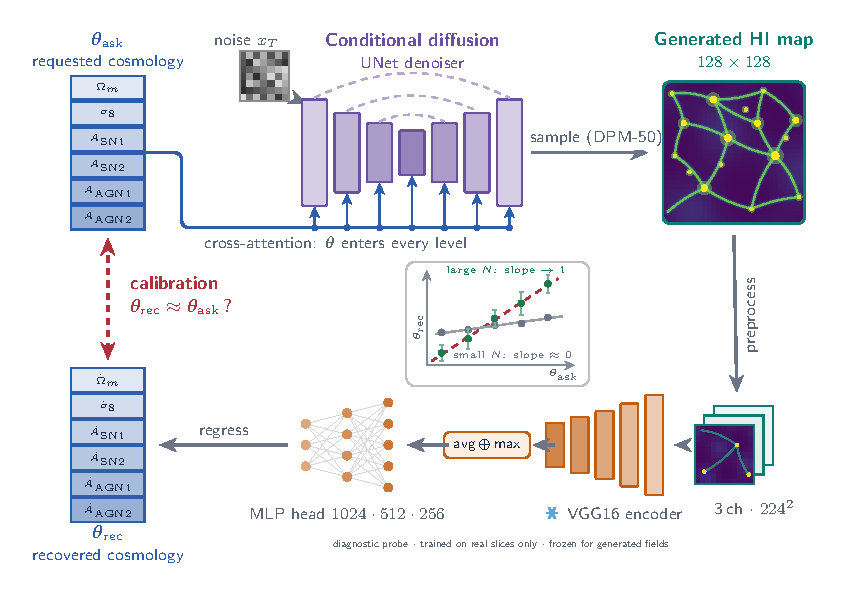
\includegraphics[width=25.2cm]{figs/calibration_roadmap_v2.pdf}
\end{center}

\SmallFont\color{subgray}
Probe safeguards: VGG16 frozen (ImageNet); regression head trained on
\emph{real} slices from non-held-out simulations only; held-out sims 900--931
used exclusively for testing and calibration.
\end{tcolorbox}

\begin{tcolorbox}[secbox={diffPurple}{Memorization $\to$ generalization transition}]
\figslot{29.0cm}{13.2cm}{nf_generalize_fig2_poster_pca_generalization_q95_serif_clean.png}
  {quickcheck notebook $\to$ PCA generalization curves with q95 threshold}

\vspace{2mm}
\begin{itemize}[leftmargin=11mm, itemsep=2mm, label=\textcolor{diffPurple}{$\blacktriangleright$}]
\item Score uses a \textbf{q95-calibrated threshold}
      ($\tau$ = 95th pct train--train NN similarity): higher means
      generated fields are less training-set-like in PCA space.
\item \textbf{Small $N_{2D}$}: generated maps remain close to training fields.
\item \textbf{Larger $N_{2D}$}: UNet-64\,/\,128\,/\,256 move toward novel
      samples; the wider UNet-256 transition is shifted to larger data.
\end{itemize}
\end{tcolorbox}

\end{minipage}\hfill
\begin{minipage}[t]{\colw}\vspace{0pt}
% ----------------------------------------------------------- COL 3

\begin{tcolorbox}[secbox={vggOrange}{Calibration results}]
\begin{center}
\figslot{28.0cm}{18.6cm}{vgg_plot.png}
  {VGG notebook $\to$ recovered vs requested $\Omega_m$ bias probe}
\end{center}

\vspace{1mm}
\SmallFont
\hl{vggOrange}{Main result:} $\Omega_m$ recovery is much flatter under
memorization (\textbf{slope 0.26}, $N_{2D}=2^7$) than in the high-data regime
(\textbf{slope 0.79}, $N_{2D}=2^{14}$). Error bars are the 16--84 percentile
spread over generated seeds at fixed $\bm{\theta}_{\rm ask}$. We lead with
$\Omega_m$ because the real-held-out VGG probe is strongest there
($R^2=0.91$; $\sigma_8=0.74$, feedback parameters weaker).
\end{tcolorbox}

\begin{tcolorbox}[secbox={fieldTeal}{Physical fidelity}]
\begin{center}
\figslot{29.0cm}{9.8cm}{fidelity_onepoint_pk.png}
  {quickcheck notebook $\to$ one-point PDF and $P(k)$ ratio comparison}
\end{center}
\vspace{1mm}
\SmallFont
In high-data examples, the one-point PDFs overlap the real reference and the
mean $P(k)$ ratio is mostly within $\sim20\%$ over the resolved $k$ range.
Intermediate undertrained runs visibly fail this check, so novelty alone is
not enough: generalization must also preserve field statistics.
\end{tcolorbox}

\begin{tcolorbox}[secbox={loopRed}{Takeaways}]
\begin{enumerate}[leftmargin=14mm, itemsep=2.5mm, label=\textcolor{loopRed}{\textbf{\arabic*.}}]
\item \textbf{Memorization is detectable.} Nearest-neighbor and
      reproducibility tests locate a data-size transition in CAMELS HI maps.
\item \textbf{Conditioning is recoverable.} High-data generated fields track
      $\bm{\theta}_{\rm ask}$ much better than memorization-regime fields.
\item \textbf{Fidelity requires generalization.} Useful emulators must be
      novel, statistically faithful, and calibrated before inference use.
\end{enumerate}
\end{tcolorbox}

\end{minipage}

\end{document}
